\documentclass{ieeeaccess}
\usepackage{cite}
\usepackage{amsmath,amssymb,amsfonts}
\usepackage{algorithm}
\usepackage{algorithmic}
\usepackage{graphicx}
\usepackage{textcomp}
\usepackage{float}
\usepackage{soul}
\def\BibTeX{{\rm B\kern-.05em{\sc i\kern-.025em b}\kern-.08em
    T\kern-.1667em\lower.7ex\hbox{E}\kern-.125emX}}

\newcommand{\TODO}[1]{\textcolor{red}{\textbf{TODO:} #1}}

\newlength{\xfigwd}

\begin{document}
\history{Date of publication xxxx 00, 0000, date of current version xxxx 00, 0000.}
\doi{10.1109/TQE.2020.DOI}

\title{A Differentiable Ising Module for Hybrid Quantum-Classical Neural Networks}
\author{\uppercase{Matteo Marchiori}\authorrefmark{1},
\uppercase{Emiliano Tolotti}\authorrefmark{1},
\uppercase{Daniele Franch}\authorrefmark{1},
\uppercase{Enrico Blanzieri}\authorrefmark{1},
and \uppercase{Davide Pastorello}\authorrefmark{2}}
\address[1]{Department of Information Engineering and Computer Science - University of Trento, Trento, Italy}
\address[2]{Department of Mathematics -- University of Bologna, 40126 Bologna, Italy;
TIFPA-INFN, 38123 Povo-Trento, Italy}

\markboth
{Marchiori \headeretal: A Differentiable Ising Module for Neural Networks}
{Marchiori \headeretal: A Differentiable Ising Module for Neural Networks}

\corresp{Corresponding author: Matteo Marchiori (email: matteo.marchiori03@gmail.com)}

\begin{abstract}
Ising machines and quantum annealers solve combinatorial optimization problems by searching for low-energy spin configurations. Recent work has shown that Ising energy minimization can itself serve as a trainable supervised model. We turn this model into a reusable deep learning component: a differentiable Ising module. Its forward pass calls an annealing solver to compute the ground-state energy of a parametric Ising Hamiltonian; its backward pass computes the analytic gradient with respect to the couplings from the spin configuration the solver returns. The module is therefore compatible with automatic differentiation in PyTorch. On top of it we build the \textit{Ising network}, a shallow architecture that combines several Ising modules through a trainable linear readout. We compare the single module against the network on nine UCI benchmarks, both in their original imbalanced form and in a balanced variant, and on XOR problems of growing dimensionality. The network matches or outperforms the single module on every benchmark: it removes the tendency to collapse onto one class under imbalance and captures interactions up to six dimensions, while remaining trainable within the standard PyTorch ecosystem. A final experiment trains both models on a D-Wave quantum processor and reproduces the simulated results on a reduced XOR task.
\end{abstract}

\begin{keywords}
Energy-based models, hybrid quantum-classical neural networks, Ising machines, Ising model, quantum annealing, quantum machine learning.
\end{keywords}

\titlepgskip=-15pt

\maketitle

\section{Introduction}

\IEEEPARstart{T}{he} Ising model originated as a description of interacting
spins in statistical mechanics~\cite{Ising1925,mccoy2014two,SherringtonKirkpatrick1975}, but it
applies well beyond magnetism: a large class of combinatorial
optimization problems can be written as the search for the lowest-energy
configuration of a spin system, and many NP-hard problems admit a direct
Ising formulation~\cite{Lucas2014ising,barahona1982computational,kalinin2022computational}.
This observation motivates the
construction of \emph{Ising machines}, devices and algorithms built
specifically to minimize an Ising energy~\cite{Mohseni2022ising,gao2024photonic}. A problem
is encoded in the local fields and pairwise couplings of the spins, and the
machine returns a low-energy configuration as a candidate solution.
Implementations range from simulated annealing~\cite{Kirkpatrick1983sa}
to dedicated physical hardware.

Quantum annealing is a general paradigm for solving such problems on quantum
hardware. The idea, introduced for the transverse-field Ising model
by~\cite{KadowakiNishimori1998}, is to evolve a quantum system slowly from
the ground state of a simple Hamiltonian toward that of the problem
Hamiltonian, so that the measured spin configuration approximates the
optimum~\cite{farhi2000quantum,das2008colloquium,mcgeoch2022adiabatic}.
Quantum annealers are the hardware realization of this paradigm; the D-Wave
Ocean SDK~\cite{DWaveOcean} exposes one such device through
a software interface, and embedding an all-to-all problem onto the sparse
qubit graph carries an additional overhead. Annealing-based solvers have been
applied across scheduling, routing, sampling and constraint satisfaction,
which makes the Ising minimization a reusable primitive rather than a
problem-specific technique.

In parallel, machine learning has become a natural target for these solvers.
Classical neural networks remain the dominant paradigm for supervised
learning~\cite{Alzubaidi2021dl}, and a substantial body of work asks how
quantum resources can play a comparable role. One direction trains
parameterized quantum circuits as differentiable models~\cite{Benedetti2019pqc,schuld2015introduction,dunjko2018machine},
optimized by gradient descent through the parameter-shift
rule~\cite{Mitarai2018qcl,wierichs2022general,pastorello2023concise}; these range from circuit-based quantum neural
networks to quantum perceptrons realized on actual
hardware~\cite{Tacchino2019neuron}, and to hybrid classical-quantum models
that interleave quantum layers with ordinary neural
networks~\cite{Mari2020transfer}. A second direction uses annealers directly,
either to train classifiers~\cite{willsch2020support,date2021qubo} or, closer to our setting, to sample from
energy-based models in the spirit of Boltzmann machines~\cite{Amin2018qbm}.
In both cases, the learning scheme must be realizable on present-day
noisy intermediate-scale quantum hardware.

Schmid, Zardini and
Pastorello~\cite{10.21468/SciPostPhysCore.7.1.013} took a more direct route:
they showed that the Ising energy minimization can itself serve as a
parametric supervised model, with the data entering as local fields, the
couplings acting as trainable weights, and the ground-state energy as the
output. The model is trained by gradient descent, and the gradients are
estimated from the spin configurations returned by the machine rather than
computed by explicit backpropagation. A useful consequence is that the
systematic error of an approximate solver is partly absorbed during training.
What that work leaves open is how to use such a model as an ordinary building
block inside the deep learning ecosystem, where layers are composed freely
and trained by automatic differentiation.

This paper addresses that gap. We recast the parametric Ising model as a
differentiable module that exposes a forward and a backward interface and
plugs directly into PyTorch. The forward pass calls an annealing solver to
estimate the ground-state energy of the spin system; the backward pass
propagates gradients to the couplings through the analytic expression of
Schmid et al., evaluated on the stored spin configurations. Because the
module behaves like any other layer, it inherits the surrounding toolchain:
optimizers, loss functions, learning-rate schedulers, mini-batching and GPU
tensors. On top of it we build the \textit{Ising network}, a shallow
architecture in which several Ising modules run in parallel and are combined
by a trainable linear readout.

The contribution of this work is threefold. First, we introduce a
differentiable Ising energy module that carries the analytic coupling
gradient into automatic differentiation, turning an Ising solver into a
standard trainable layer. Second, we propose the Ising network, a hybrid
architecture that assembles a set of energy-based units into a single
trainable layer through a linear readout. Third, we report an empirical study
on nine UCI benchmarks, evaluated both in their native class-imbalanced form
and in a pre-balanced variant, and on a family of synthetic XOR problems of
growing dimensionality, comparing the single module against the network,
together with a first run of both models on a D-Wave quantum processor.

The remainder of the paper is organized as follows.
Section~\ref{sec:background} reviews the background: the Ising model, its
realization through quantum annealing, and the parametric learning model of
Schmid et al., including its analytic gradients and the offset scheme for
hidden spins. Section~\ref{sec:proposal} presents our proposal, namely the
differentiable Ising module and the Ising network built on top of it.
Section~\ref{sec:empirical} describes the experimental setup and reports the
results on the UCI and XOR benchmarks, including a run on quantum hardware.
Section~\ref{sec:discussion} discusses
these findings and Section~\ref{sec:conclusion} concludes.

\section{Background}\label{sec:background}
This section collects the background our method builds on: the Ising model,
its realization through quantum annealing, and the parametric learning model
of Schmid et al.~\cite{10.21468/SciPostPhysCore.7.1.013} on which the
differentiable module rests.

\subsection{The Ising Model}
The Ising model was introduced to describe ferromagnetic
systems~\cite{Ising1925} and has since become a standard
framework in statistical mechanics. It is defined on a graph \( (V, E) \),
where each vertex \( i \in V \) carries a discrete spin variable
\( z_i \in \{-1, +1\} \). Each spin has a local bias \( \theta_i \in \mathbb{R} \),
and each edge \( (i, j) \) a pairwise coupling \( \Gamma_{ij} \in \mathbb{R} \).
The total energy of a configuration is given by the Hamiltonian:
\begin{equation}\label{eq:ising}
    E(\theta, \Gamma, z) = \sum_{i \in V} \theta_i z_i + \sum_{(i,j) \in E} \Gamma_{ij} z_i z_j.
\end{equation} 

An Ising machine seeks the spin configuration that minimizes this Hamiltonian:
\begin{equation}
z^* = \arg\min_z E(\theta, \Gamma, z),
\end{equation}
where $z^*$ is the ground-state configuration. Because many discrete problems
admit an Ising formulation~\cite{Lucas2014ising}, this minimization encodes a
wide class of combinatorial optimization tasks, and devices built to perform
it Ising machines range from digital simulated
annealing~\cite{Kirkpatrick1983sa} to coherent optical machines and quantum
annealers~\cite{Mohseni2022ising}.

\begin{figure}[t]
    \centering
    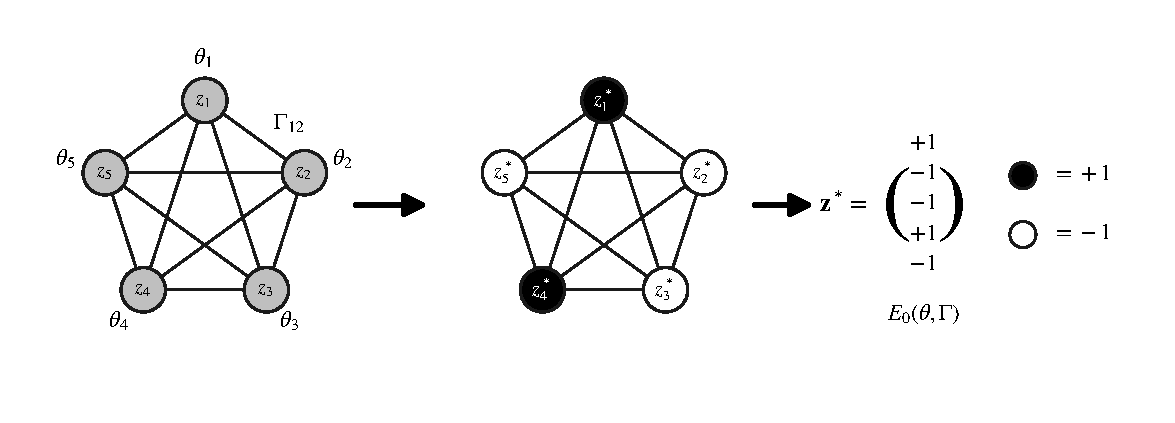
\includegraphics[width=\linewidth]{plots/ising_model.pdf}
    \caption{On the left, an Ising model on a fully connected graph with
        \( |V| = 5 \) spins \( z \), biases \( \theta \) and couplings
        \( \Gamma \). On the right, the output of an Ising machine: a
        \(\{-1, +1\}\) assignment (white/black nodes) for each spin, that is,
        the configuration \( z^{*} \) together with its minimal energy
        \( E_{0}(\theta, \Gamma) \). Adapted
        from~\cite{10.21468/SciPostPhysCore.7.1.013}.
    }
    \label{fig:isingModel}
\end{figure}

\subsection{Quantum Annealing}
Quantum annealing solves optimization problems by evolving a quantum system
toward the ground state of a problem Hamiltonian~\cite{KadowakiNishimori1998}.
The Ising minimization of Eq.~\ref{eq:ising} maps to the ground-state search
of a corresponding Hamiltonian. Consider the time-dependent Hamiltonian
\begin{equation}
    H(t) = \gamma(t) H_D + H_P
\end{equation}
where $H_P$ is the problem Hamiltonian, $H_D$ is the transverse-field
Hamiltonian, and $\gamma : \mathbb{R}^+ \to \mathbb{R}$ is a decreasing
function that gradually suppresses the kinetic term $H_D$, guiding the system
toward the ground state of $H_P$. The transverse field provides the quantum
fluctuations that let the system explore the solution landscape.

Quantum annealing is realized physically on a network of qubits placed on the
vertices of a graph $(V, E)$, with $|V| = n$, whose edges $E$ carry the
couplings between qubits. The problem Hamiltonian is a self-adjoint operator
on the $n$-qubit Hilbert space $\left(\mathbb{C}^2\right)^{\otimes n}$:
\begin{equation}
H_P = \sum_{i \in V} \theta_i \, \sigma_z^{(i)} + \sum_{(i,j) \in E} \Gamma_{ij} \, \sigma_z^{(i)} \sigma_z^{(j)},
\label{hamiltonian}
\end{equation}
where $\sigma_z^{(i)}$ is the Pauli-$z$ operator acting on qubit $i$, and
$\theta_i$ and $\Gamma_{ij}$ are the local fields and the couplings between
qubits. The transverse-field Hamiltonian is the sum of the Pauli-$x$
operators on the same qubits,
\begin{equation}
H_D = - \sum_{i \in V} \sigma_x^{(i)},
\label{eq:driver}
\end{equation}
whose ground state is the uniform superposition of all the spin
configurations. Quantum annealing is therefore a physical mechanism for minimizing
the Ising Hamiltonian. The D-Wave processors implement this scheme on a sparse
hardware graph, so mapping a fully connected problem requires an embedding
step with an additional overhead~\cite{DWaveOcean}.

\subsection{Parametric Model}\label{sec:parametric}
Schmid et al.~\cite{10.21468/SciPostPhysCore.7.1.013} turned the Ising
minimization into a supervised learning model. The model is defined as
\begin{align}
F(\boldsymbol{\theta}|\Gamma, \lambda, \varepsilon) &= \lambda \min_{\mathbf{z} \in \{-1,1\}^n} E(\boldsymbol{\theta}, \Gamma, \mathbf{z}) + \varepsilon \\
&= \lambda E_0(\boldsymbol{\theta}, \Gamma) + \varepsilon.
\label{model}
\end{align}
The input data enter as the spin biases $\boldsymbol{\theta} = (\theta_1, \ldots, \theta_n)$,
the couplings $\Gamma_{ij}$ on the topology of the Ising machine are the
trainable weights, and the output is the ground-state energy
$E_0(\boldsymbol{\theta}, \Gamma)$, rescaled by $\lambda$ and shifted by
$\varepsilon$. The two additional parameters let the model match the range of
the target outputs, playing a role comparable to the weight and the bias of a
linear layer. The arrangement is neural-like: spins play the
role of neurons and couplings that of synaptic weights.

\subsubsection{Training Phase}\label{sec:training_bg}

Given a training set $\mathcal{D} = \{(\boldsymbol{\theta}^{(a)}, y^{(a)})\}_{a=1,\ldots,N}$
with $y^{(a)} = f(\boldsymbol{\theta}^{(a)})$, where $f : \mathcal{X} \rightarrow \mathbb{R}$
is the unknown target, the model~\eqref{model} is trained by minimizing a
loss function, for example the mean squared error (MSE),
\begin{equation}
L(\Gamma, \lambda, \varepsilon) = \frac{1}{N} \sum_{a=1}^{N}
\left[ F(\boldsymbol{\theta}^{(a)} | \Gamma, \lambda, \varepsilon) - y^{(a)} \right]^2,
\label{eq:loss}
\end{equation}
by gradient descent, updating each parameter against the gradient of $L$:
\begin{equation}
\delta \Gamma = -\eta \nabla_{\Gamma} L, \quad
\delta \lambda = -\eta \frac{\partial L}{\partial \lambda}, \quad
\delta \varepsilon = -\eta \frac{\partial L}{\partial \varepsilon},
\label{eq:gradients}
\end{equation}
with learning rate $\eta > 0$.

The key observation of~\cite{10.21468/SciPostPhysCore.7.1.013} is that these gradients
need no explicit backpropagation through the minimization: they are read off
the spin configuration $z^*$ the machine already returns.
Differentiating
$F = \lambda E_0 + \varepsilon$ and using $E_0 = \sum_i \theta_i z^*_i + \sum_{(i,j)} \Gamma_{ij} z^*_i z^*_j$,
the partial derivatives are
\begin{equation}
\frac{\partial F}{\partial \Gamma_{ij}} = \lambda\, z^*_i z^*_j, \qquad
\frac{\partial F}{\partial \lambda} = E_0(\boldsymbol{\theta}, \Gamma), \qquad
\frac{\partial F}{\partial \varepsilon} = 1.
\label{eq:partials}
\end{equation}
In particular $\partial E_0 / \partial \Gamma_{ij} = z^*_i z^*_j$, so a single
call to the machine yields both the prediction $E_0$ and the quantities needed
to update the couplings. Schmid et al. prove that the derivatives of
Eq.~\eqref{eq:partials} are well defined almost everywhere in the parameter
space~\cite{10.21468/SciPostPhysCore.7.1.013}. Training
therefore mirrors that of a neural network, with the conventional
backpropagation step replaced by the Ising-machine evaluation of $E_0$ and
$z^*$. A practical benefit is that exact ground states are not required: the
systematic deviations of an approximate solver are absorbed by the parameter
updates, which makes the scheme usable with real annealers.


\subsubsection{Hidden Spins}\label{sec:hidden_spins}

On a complete topology the number of couplings $\Gamma_{ij}$ grows
quadratically with the input dimension $n$, so the model capacity is fixed by
the dimensionality of the data, much like a neural network with only an input
and an output layer. To add capacity, Schmid et al. introduce \emph{hidden
spins}: extra nodes in the topology graph that contribute additional couplings
and hence additional parameters. They are obtained through a preprocessing
map
\begin{equation}
h_{\mathrm{pre}} : \mathbb{R}^n \to \mathbb{R}^{n_{\mathrm{total}}},
\qquad n_{\mathrm{total}} = n + n_{\mathrm{hidden}},
\label{eq:hpre}
\end{equation}
that lifts the input $\boldsymbol{\theta}$ from the feature space into a
higher-dimensional space before it is fed to the Ising model. The map does not
change the training procedure of Section~\ref{sec:training_bg}, but its choice
matters. Padding with zeros, for instance, makes the hidden spins
indistinguishable and therefore redundant, while filling them with random
values risks overshadowing the original input when
$n_{\mathrm{hidden}} \gg n$.

The scheme adopted in~\cite{10.21468/SciPostPhysCore.7.1.013} is a constant
real-valued \emph{offset} initialization,
\begin{equation}
\boldsymbol{\theta} \in \mathbb{R}^n \;\mapsto\;
h_{\mathrm{offset}}(\boldsymbol{\theta}) =
\begin{pmatrix}
\boldsymbol{\theta} \\
\boldsymbol{\theta} + 1 \cdot \mathbf{d} \\
\vdots \\
\boldsymbol{\theta} + (l-1)\cdot \mathbf{d}
\end{pmatrix}
\in \mathbb{R}^{n_{\mathrm{total}}},
\label{eq:offset}
\end{equation}
with $\mathbf{d} \in \mathbb{R}^n$, $l \in \mathbb{Z}^+$ and
$n_{\mathrm{total}} = l\,n$. The input is concatenated with itself $l$ times,
each copy shifted by an increasing multiple of the offset $\mathbf{d}$, so that
the hidden spins start from distinct biases yet stay tied to the original
features. In the reference implementation
of~\cite{10.21468/SciPostPhysCore.7.1.013} the offset $\mathbf{d}$ is a single
scalar $\varepsilon_h$ added to every component, and $n_{\mathrm{total}}$ need
not be a multiple of $n$: the copies are tiled cyclically and the last one is
truncated to match the annealer size. This is the hidden-spin scheme we reuse
unchanged in the differentiable module of Section~\ref{sec:proposal}.


\section{Differentiable Ising Modules and Networks}\label{sec:proposal}

The parametric model of Section~\ref{sec:parametric} is trained with the
hand-coded update rules of Eq.~\eqref{eq:partials}, outside any
deep-learning framework. We turn it into a reusable component. Our
contribution is twofold: a differentiable \emph{Ising module} that wraps the
annealing call and the analytic coupling gradient into a single autograd
primitive, and the Ising network, a shallow architecture that composes
several such modules. The gradient formulas are those recalled in
Section~\ref{sec:training_bg}; what is new here is the construction that makes
them interoperable with automatic differentiation and the architecture built
on top.

\subsection{The Ising Module}

\subsubsection{Motivation}

Automatic differentiation requires every operation in the computational graph
to expose a backward rule. The ground-state map $\boldsymbol{\theta} \mapsto E_0$
does not: it contains a minimization over the discrete set $\{-1,+1\}^n$,
which is not differentiable and is, moreover, computed by an external solver
that the framework cannot trace. The model of Schmid et al. sidesteps this
through the analytic derivatives of Eq.~\eqref{eq:partials}, but those were
applied by explicit update rules. The module below carries the same
derivatives into a standard autograd primitive, so that an Ising solver can be
dropped into a network and trained like any other layer.

\subsubsection{Differentiable Ising Energy Function}

We implement the ground-state energy as a custom autograd function with a
forward and a backward rule. In the forward pass, for each input vector
$\boldsymbol{\theta}$ in the batch the annealer returns an approximate
ground-state configuration $z^*$ and the corresponding energy
$E_0(\boldsymbol{\theta}, \Gamma)$ of Eq.~\eqref{model}; the configuration
$z^*$ is cached for the backward pass. In the backward pass we use the
analytic derivative of Eq.~\eqref{eq:partials},
\[
\frac{\partial E_0}{\partial \Gamma_{ij}} = z_i^* z_j^*,
\]
evaluated on the cached $z^*$, and combine it with the incoming gradient
$\partial L / \partial E_0$ by the chain rule.
The backward rule also returns the envelope-theorem gradient with respect to
the input biases, $\partial E_0 / \partial \theta_i = z^*_i$, so the function
can be composed with upstream layers; in the experiments of this paper,
however, $\boldsymbol{\theta}$ carries the raw data and only the couplings
$\Gamma$ are trained through this function. No gradient flows through the
annealer itself: the returned spin configurations are treated as constants.
With both rules in place, the
energy minimization behaves as an ordinary node of a PyTorch graph.
Algorithm~\ref{alg:energy_function} summarizes the two passes.

\begin{algorithm}[H]
\caption{Differentiable Ising Energy Function (Forward and Backward)}
\label{alg:energy_function}
\begin{algorithmic}[1]
\STATE \textbf{Input:} batch of biases $\{\theta_i\}$, coupling matrix $\Gamma$, annealer instance
\STATE \textbf{Forward pass:}
\FOR{each sample $i$ in batch, in parallel across workers}
    \STATE Query the annealer with $(\theta_i, \Gamma)$: obtain the approximate ground state $z_i^*$ and its energy $E_i$
    \STATE Store $z_i^*$ for backward
\ENDFOR
\STATE \textbf{Return:} batch energies $\{E_i\}$
\STATE \textbf{Backward pass:}
\FOR{each sample $i$ in batch}
    \STATE Compute outer product $z_i^* (z_i^*)^\top$
    \STATE Multiply by incoming gradient $\partial L / \partial E_i$
\ENDFOR
\STATE Sum over batch and retain the strictly upper-triangular part to get $\partial L / \partial \Gamma$
\STATE \textbf{Return:} $\partial L / \partial \Gamma$
\end{algorithmic}
\end{algorithm}

\subsubsection{The Ising Module}

The Ising module wraps this function and adds the two learnable parameters of
the parametric model, the scale $\lambda$ and the offset $\varepsilon$, so
that its output is
\[
F(\boldsymbol{\theta}) = \lambda\, E_0(\boldsymbol{\theta}, \Gamma) + \varepsilon.
\]
The scale and offset let the module match the range of the target outputs,
playing a role comparable to the weight and bias of a linear layer. All three
quantities $\Gamma$, $\lambda$ and $\varepsilon$ are registered as
parameters and updated by the surrounding optimizer, so the module trains
end-to-end. Algorithm~\ref{alg:module_forward} summarizes the forward pass.

\begin{algorithm}[H]
\caption{Forward Pass of the Ising Module}
\label{alg:module_forward}
\begin{algorithmic}[1]
\STATE Compute $E_0$ using the Ising Energy Function
\STATE Scale and shift: $F = \lambda \cdot E_0 + \varepsilon$
\STATE \textbf{Return:} $F$
\end{algorithmic}
\end{algorithm}

\subsubsection{Parallelized Computation}

The annealing call dominates the cost of the forward pass, and the calls for
different samples are independent. We exploit this by splitting the batch
across a pool of worker threads, each holding its own sampler instance and
solving a disjoint subset of the inputs. This keeps the wall-clock cost of
embedding an Ising solver in a network manageable on multicore hardware.

\subsection{The Ising Network}\label{sec:singlelayer}

A single module exposes one coupling matrix and one ground-state energy. To
add capacity, we place $M$ Ising modules in parallel and combine their outputs
with a trainable linear readout; the result is the Ising network, a
single-layer architecture in which each unit is an independent Ising model.

\begin{figure}[t]
    \centering
    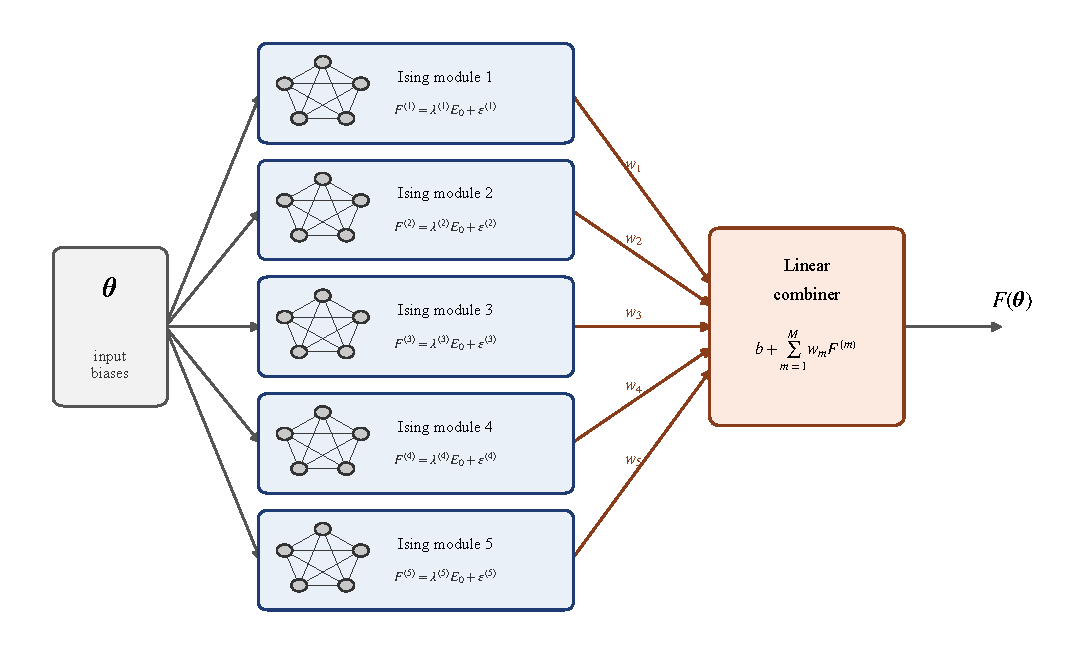
\includegraphics[width=\linewidth]{plots/multiising_network.pdf}
    \caption{Schematic of the Ising network. The input biases
    $\boldsymbol{\theta}$ are shared across $M=5$ parallel Ising modules, each
    one an Ising model whose spins and pairwise couplings $\Gamma^{(m)}$ are
    drawn as a small fully connected graph. Every module returns a scalar
    $F^{(m)}=\lambda^{(m)}E_0+\varepsilon^{(m)}$, and the trainable linear
    combiner aggregates these outputs as $b+\sum_{m} w_m F^{(m)}$ to produce
    the network output $F(\boldsymbol{\theta})$.
    }
    \label{fig:multiising_nn}
\end{figure}

Given an input vector $\boldsymbol{\theta}$, the $m$-th module produces
\begin{equation}
F^{(m)}(\boldsymbol{\theta}) \;=\; \lambda^{(m)} \, E_0\!\big(\boldsymbol{\theta}, \Gamma^{(m)}\big) \;+\; \varepsilon^{(m)},
\label{eq:fullising_out}
\end{equation}
with its own couplings $\Gamma^{(m)}$ and its own scale and offset
$\lambda^{(m)}, \varepsilon^{(m)}$. The $M$ outputs are aggregated by a linear
readout,
\begin{equation}
F(\boldsymbol{\theta}) \;=\; b \;+\; \sum_{m=1}^{M} w_m \, F^{(m)}(\boldsymbol{\theta}),
\label{eq:linear_comb_fullising}
\end{equation}
with trainable weights $w_m$ and bias $b$.

The construction mirrors a single fully connected layer, except that each
neuron is an Ising module: the nonlinearity comes from the discrete
ground-state computation inside each unit, and the linear readout combines the
resulting energy-based features. Even though the architecture stays shallow,
distinct modules can settle on different coupling patterns, which gives the
network more expressive power than a single module.

\section{Empirical Evaluation}\label{sec:empirical}

We compare the single Ising module with the Ising network, $M=5$ parallel
modules aggregated through a linear readout. The evaluation is split in three
blocks. The first uses nine UCI benchmarks in their native form, which for
most of them is class-imbalanced. The second runs the same pipeline on a
pre-balanced variant of those datasets, removing the class prior. The third
uses synthetic $d$-dimensional XOR problems as a controlled probe of
non-linear capacity. The two UCI blocks share the datasets, the training
pipeline and the hyperparameters and differ only in data preparation, which
separates the effect of class imbalance from that of model capacity; the XOR
block then probes the architectural gap between the two models. A final
experiment repeats the 2D XOR comparison on a D-Wave quantum processor.

\subsection{Method}\label{sec:method}

\subsubsection{Datasets}\label{sec:datasets}

We adopt nine binary classification datasets from the UCI Machine Learning
Repository~\cite{Dua:2019}, spanning feature dimensionalities from 3 to 44 and
sample sizes from 100 to 1\,372. The UCI suite is
complemented by a family of synthetic $d$-dimensional XOR datasets for
$d \in \{1,\dots,6\}$, a controlled stress test for higher-order non-linear
interactions. Table~\ref{tab:datasets} summarizes the size and per-class
distribution of both groups.

\begin{table}[H]
\centering
\caption{Summary of the datasets used in the experimental evaluation.}
\label{tab:datasets}
\begin{tabular}{lccc}
\hline
Dataset                         & \# Features & \# Samples & Class dist.\ (0/1) \\
\hline
00\_iris\_versicolor\_virginica & 4           & 100          & 50 / 50      \\
01\_vertebral\_column           & 6           & 200         & 100 / 100    \\
02\_banknote                    & 4           & 1372        & 762 / 610    \\
03\_breast\_cancer              & 30          & 569         & 357 / 212    \\
04\_contraceptive\_method       & 9           & 962         & 629 / 333    \\
05\_haberman\_survival          & 3           & 306         & 225 / 81     \\
06\_heart\_failure              & 12          & 299         & 203 / 96     \\
07\_ionosphere                  & 34          & 351         & 126 / 225    \\
08\_SPECTF\_Heart               & 44          & 267         & 55 / 212     \\
\multicolumn{4}{c}{\textit{Synthetic XOR datasets}} \\
XOR-1D                          & 1           & 200         & 100 / 100    \\
XOR-2D                          & 2           & 400         & 200 / 200    \\
XOR-3D                          & 3           & 800         & 400 / 400    \\
XOR-4D                          & 4           & 1600        & 800 / 800    \\
XOR-5D                          & 5           & 3200        & 1600 / 1600  \\
XOR-6D                          & 6           & 6400        & 3200 / 3200  \\
\hline
\end{tabular}
\end{table}

\subsubsection{Evaluation Protocol}\label{sec:evalprotocol}

UCI performance is assessed under two complementary forms that share
the same model, training pipeline and hyperparameters, and differ only
in how the data fed to the cross-validation procedure is constructed.

\paragraph{Original (imbalanced) datasets} Each UCI dataset is used
in its native form, with the class distribution reported in
Table~\ref{tab:datasets}. Stratified 5-fold cross-validation preserves the
original class ratios, so the training and test splits keep the native
distribution. This form measures how the two architectures behave
when no class-balancing intervention is applied.

\paragraph{Pre-balanced fixed folds (random subsampling)} For each UCI
dataset a class-balanced variant is prebuilt by random undersampling
of the majority class, and the resulting CSV is stored on disk. The
same stratified 5-fold splitter is then applied to the already balanced
files, so every fold contains an equal number of class~0 and class~1
samples in both the training and the test split. Because the folds are
produced from a fixed file and the random seed is fixed
(Table~\ref{tab:hyperparameters}), the splits are deterministic and
shared across the two architectures.

\paragraph{Shared protocol} In both forms, feature standardization is
fit on the training fold only and applied to the test fold (preventing
information leakage), the random seed is held fixed across runs, and
five metrics are collected and averaged across folds: classification
accuracy, precision, recall, $F_1$ score, and area under the ROC curve
(AUC). For the synthetic XOR problems we use a single stratified 80/20
train/test split with the same training pipeline as the UCI experiments.

\subsubsection{Training and Inference Procedure}\label{sec:training}

The training phase is implemented in PyTorch. Both architectures are
trained with the Adam optimizer and the binary cross-entropy with
logits loss (\texttt{BCEWithLogitsLoss}), for a fixed number of epochs
with mini-batch gradient descent. At inference time the sigmoid
activation is applied to the logits to obtain class probabilities, and
a threshold of $0.5$ is used for binary classification.

\subsubsection{Hyperparameter Configuration}\label{sec:hyperparams}

A single set of hyperparameters is shared across all UCI and XOR
experiments (Table~\ref{tab:hyperparameters}). The values were chosen to
give stable performance across the considered benchmarks rather than
tuned per architecture or per dataset, so that the comparison reflects
architectural differences and not per-task hyperparameter gains.

\begin{table}[H]
\centering
\caption{Hyperparameters used in all experiments. Values are shared between
the single Ising module and the Ising network; the combiner learning rate
applies to the Ising network only, and the K-Fold cross-validation is used on
the UCI benchmarks only.}
\label{tab:hyperparameters}
\begin{tabular}{ll}
\hline
Hyperparameter                                  & Value \\
\hline
\multicolumn{2}{l}{\textit{Optimization}} \\
Optimizer                                       & Adam \\
Loss                                            & \texttt{BCEWithLogitsLoss} \\
Number of epochs                                & 200 \\
Batch size                                      & 32 \\
K-Folds (UCI only)                              & 5 \\
Random seed                                     & 42 \\
\hline
\multicolumn{2}{l}{\textit{Per-parameter learning rates}} \\
$\eta_{\Gamma}$ (couplings)                     & $1\!\times\!10^{-3}$ \\
$\eta_{\lambda}$ (energy scale)                 & $5\!\times\!10^{-3}$ \\
$\eta_{\varepsilon}$ (offset)                   & $1\!\times\!10^{-2}$ \\
$\eta_{\text{comb}}$ (linear combiner)          & $5\!\times\!10^{-3}$ \\
\hline
\multicolumn{2}{l}{\textit{Architecture}} \\
Annealer size $n$                               & 50 spins \\
Ising modules $M$ (Ising network)               & 5 \\
Partition input across modules                  & False (full input replicated) \\
Hidden-nodes offset $\varepsilon_h$             & $-0.02$ \\
$\Gamma$ initialization                         & $0.0$ \\
$\lambda$ initialization                        & $1.0$ ($\pm 0.1$) \\
$\varepsilon$ initialization                    & $1.0$ ($\pm 0.1$) \\
\# trainable parameters (single Ising module)   & 1\,227 \\
\# trainable parameters (Ising network)         & 6\,141 \\
\hline
\multicolumn{2}{l}{\textit{Simulated annealing}} \\
Inverse temperature $\beta$ range               & $[1,\,10]$ \\
Number of reads                                 & 1 \\
Number of sweeps                                & 1\,000 \\
Sweeps per $\beta$ step                         & 1 \\
\hline
\end{tabular}
\end{table}


\subsection{Results}\label{sec:results}

\subsubsection{Native (Imbalanced) UCI Benchmarks}\label{sec:res_imbalanced}

Tables~\ref{tab:ising_uci_imbalanced} and~\ref{tab:nn_uci_imbalanced}
collect the per-dataset metrics for the single module and the network.
Measured by AUC, the network matches or exceeds the single module on every
benchmark, with the widest gaps on breast cancer, banknote and heart failure.
The difference between the two models lies less in the final accuracy than in
how they reach it. On four datasets the single module stops separating the classes and
collapses onto a single label. On breast cancer, haberman and heart failure it
predicts almost exclusively the negative class, so precision, recall and $F_1$
drop to or near zero while accuracy merely tracks the share of negative samples; on
SPECTF the collapse goes the other way, with the module predicting only the
positive class, which gives a recall of one and a precision equal to the
positive-class frequency. On haberman and heart failure this single-label
behaviour even pushes the module's accuracy above that of the network, even
though the classes are not actually separated. The network shows no such
collapse on any of these datasets.

Several entries in
Table~\ref{tab:ising_uci_imbalanced} look strong at first glance, but they
do not reflect genuine class separation. When a binary classifier
defaults to predicting the majority label, its accuracy mechanically
matches the class prior; the rows in which precision and recall
collapse make this pattern explicit. The balanced form in
Section~\ref{sec:res_balanced} removes this shortcut and provides a
cleaner view of what each model actually learns.

\begin{table}[H]
\centering
\caption{Single Ising module on the UCI datasets in the imbalanced form. 5-fold CV, mean $\pm$ std.}
\label{tab:ising_uci_imbalanced}
\resizebox{\linewidth}{!}{%
\begin{tabular}{lccccc}
\hline
Dataset                         & Accuracy          & Precision         & Recall            & $F_1$             & AUC               \\
\hline
iris (versicolor/virginica)     & $0.72 \pm 0.11$ & $0.74 \pm 0.10$ & $0.68 \pm 0.20$ & $0.70 \pm 0.14$ & $0.76 \pm 0.14$ \\
vertebral column                & $0.73 \pm 0.05$ & $0.71 \pm 0.07$ & $0.78 \pm 0.09$ & $0.74 \pm 0.05$ & $0.80 \pm 0.05$ \\
banknote                        & $0.71 \pm 0.02$ & $0.68 \pm 0.04$ & $0.67 \pm 0.11$ & $0.66 \pm 0.05$ & $0.72 \pm 0.02$ \\
breast cancer                   & $0.63 \pm 0.00$ & $0.00 \pm 0.00$ & $0.00 \pm 0.00$ & $0.00 \pm 0.00$ & $0.50 \pm 0.06$ \\
contraceptive method            & $0.69 \pm 0.03$ & $0.59 \pm 0.07$ & $0.40 \pm 0.12$ & $0.47 \pm 0.10$ & $0.72 \pm 0.04$ \\
haberman                        & $0.74 \pm 0.00$ & $0.00 \pm 0.00$ & $0.00 \pm 0.00$ & $0.00 \pm 0.00$ & $0.52 \pm 0.07$ \\
heart failure                   & $0.68 \pm 0.00$ & $0.30 \pm 0.40$ & $0.02 \pm 0.03$ & $0.04 \pm 0.05$ & $0.42 \pm 0.11$ \\
ionosphere                      & $0.89 \pm 0.03$ & $0.89 \pm 0.04$ & $0.96 \pm 0.01$ & $0.92 \pm 0.02$ & $0.96 \pm 0.03$ \\
SPECTF                          & $0.79 \pm 0.00$ & $0.79 \pm 0.00$ & $1.00 \pm 0.00$ & $0.89 \pm 0.00$ & $0.71 \pm 0.02$ \\
\hline
\end{tabular}}
\end{table}

\begin{table}[H]
\centering
\caption{Ising network on the UCI datasets in the imbalanced form. 5-fold CV, mean $\pm$ std.}
\label{tab:nn_uci_imbalanced}
\resizebox{\linewidth}{!}{%
\begin{tabular}{lccccc}
\hline
Dataset                         & Accuracy          & Precision         & Recall            & $F_1$             & AUC               \\
\hline
iris (versicolor/virginica)     & $0.93 \pm 0.06$ & $0.92 \pm 0.10$ & $0.96 \pm 0.08$ & $0.93 \pm 0.06$ & $0.93 \pm 0.06$ \\
vertebral column                & $0.78 \pm 0.09$ & $0.80 \pm 0.09$ & $0.75 \pm 0.14$ & $0.77 \pm 0.11$ & $0.88 \pm 0.04$ \\
banknote                        & $1.00 \pm 0.00$ & $1.00 \pm 0.01$ & $1.00 \pm 0.00$ & $1.00 \pm 0.00$ & $1.00 \pm 0.00$ \\
breast cancer                   & $0.84 \pm 0.03$ & $0.81 \pm 0.08$ & $0.77 \pm 0.08$ & $0.78 \pm 0.04$ & $0.92 \pm 0.03$ \\
contraceptive method            & $0.71 \pm 0.02$ & $0.62 \pm 0.06$ & $0.48 \pm 0.13$ & $0.52 \pm 0.06$ & $0.76 \pm 0.01$ \\
haberman                        & $0.66 \pm 0.05$ & $0.26 \pm 0.10$ & $0.15 \pm 0.09$ & $0.18 \pm 0.08$ & $0.58 \pm 0.04$ \\
heart failure                   & $0.66 \pm 0.04$ & $0.48 \pm 0.07$ & $0.41 \pm 0.06$ & $0.44 \pm 0.05$ & $0.66 \pm 0.08$ \\
ionosphere                      & $0.94 \pm 0.03$ & $0.94 \pm 0.04$ & $0.97 \pm 0.02$ & $0.96 \pm 0.02$ & $0.98 \pm 0.01$ \\
SPECTF                          & $0.80 \pm 0.03$ & $0.84 \pm 0.02$ & $0.92 \pm 0.02$ & $0.88 \pm 0.02$ & $0.81 \pm 0.04$ \\
\hline
\end{tabular}}
\end{table}

Figure~\ref{fig:boxplot_imbalanced} summarizes the fold-level dispersion. The
network boxes sit at higher accuracy than the single module on most datasets,
most clearly on iris, banknote and breast cancer. On haberman, heart failure
and SPECTF the single-module box collapses to an almost flat line: the model
predicts a near-constant label, so its variance is small and, on haberman and
heart failure, this constant prediction even sits above the network.

\begin{figure}[H]
    \centering
    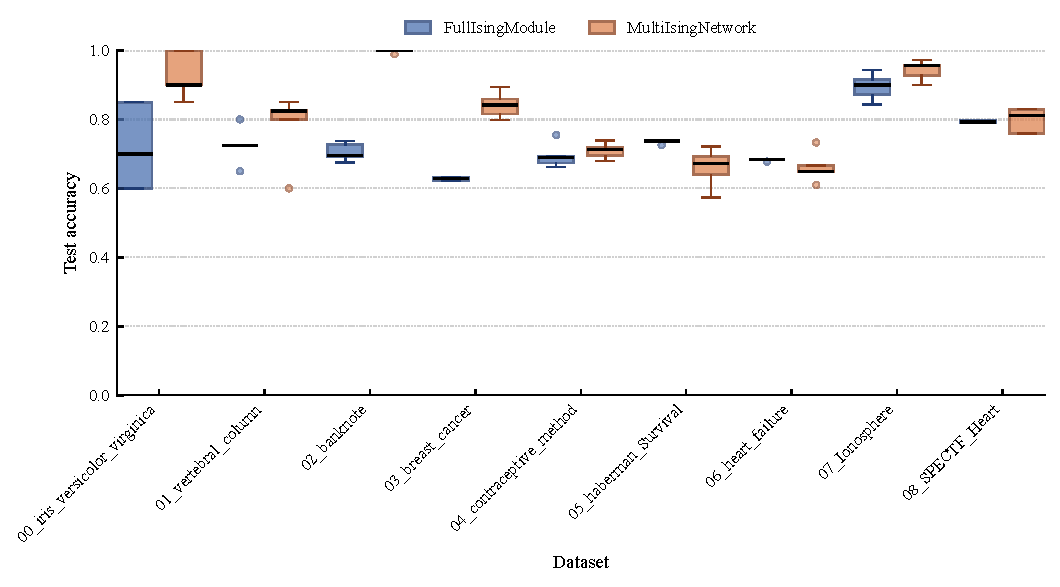
\includegraphics[width=\linewidth]{plots/uci_imbalanced_combined_boxplot.pdf}
    \caption{Test accuracy on the imbalanced UCI datasets. Each box aggregates
    the five cross-validation folds for the single Ising module and the Ising
    network.}
    \label{fig:boxplot_imbalanced}
\end{figure}

\subsubsection{Pre-balanced UCI Benchmarks}\label{sec:res_balanced}

The same comparison is repeated on the balanced variant of the nine UCI sets,
everything else held fixed. Per-dataset metrics are reported in
Tables~\ref{tab:ising_uci_balanced} and~\ref{tab:nn_uci_balanced}. Removing the
class-prior shortcut lowers the scores of both models. The drop is
larger for the single module, which loses several points of accuracy on
average, while the network keeps a clear margin on breast cancer, ionosphere,
heart failure and SPECTF. On the sets where the single module previously
collapsed to a constant predictor, precision, recall and $F_1$ are now
non-zero: balancing removes the single-label behaviour, and the margins that
remain reflect learned class separation rather than the class prior.
The
exception is haberman, where neither model exceeds chance. This matches the
literature, where haberman is reported as one of the hardest UCI benchmarks:
its minority class is dominated by borderline and rare examples lying in the
class-overlap region rather than by safe ones, a configuration known to drive
classifiers toward the majority baseline regardless of the
model~\cite{Napierala2016types}. We therefore read the haberman result as a
property of the data rather than a shortcoming of either model.

\begin{table}[H]
\centering
\caption{Single Ising module on the pre-balanced UCI datasets. 5-fold CV on the balanced files, mean $\pm$ std.}
\label{tab:ising_uci_balanced}
\resizebox{\linewidth}{!}{%
\begin{tabular}{lccccc}
\hline
Dataset                         & Accuracy          & Precision         & Recall            & $F_1$             & AUC               \\
\hline
iris (versicolor/virginica)     & $0.73 \pm 0.11$ & $0.74 \pm 0.10$ & $0.70 \pm 0.20$ & $0.71 \pm 0.14$ & $0.77 \pm 0.14$ \\
vertebral column                & $0.73 \pm 0.06$ & $0.71 \pm 0.07$ & $0.78 \pm 0.10$ & $0.74 \pm 0.06$ & $0.79 \pm 0.05$ \\
banknote                        & $0.76 \pm 0.08$ & $0.81 \pm 0.11$ & $0.71 \pm 0.17$ & $0.74 \pm 0.11$ & $0.85 \pm 0.04$ \\
breast cancer                   & $0.59 \pm 0.06$ & $0.59 \pm 0.05$ & $0.61 \pm 0.12$ & $0.60 \pm 0.07$ & $0.60 \pm 0.07$ \\
contraceptive method            & $0.65 \pm 0.06$ & $0.65 \pm 0.07$ & $0.65 \pm 0.08$ & $0.65 \pm 0.07$ & $0.72 \pm 0.05$ \\
haberman                        & $0.49 \pm 0.07$ & $0.52 \pm 0.10$ & $0.57 \pm 0.17$ & $0.52 \pm 0.07$ & $0.49 \pm 0.07$ \\
heart failure                   & $0.45 \pm 0.04$ & $0.45 \pm 0.05$ & $0.49 \pm 0.12$ & $0.46 \pm 0.08$ & $0.43 \pm 0.03$ \\
ionosphere                      & $0.58 \pm 0.04$ & $0.60 \pm 0.05$ & $0.54 \pm 0.14$ & $0.55 \pm 0.06$ & $0.62 \pm 0.05$ \\
SPECTF                          & $0.39 \pm 0.06$ & $0.41 \pm 0.06$ & $0.58 \pm 0.17$ & $0.47 \pm 0.10$ & $0.20 \pm 0.01$ \\
\hline
\end{tabular}}
\end{table}

\begin{table}[H]
\centering
\caption{Ising network on the pre-balanced UCI datasets. 5-fold CV on the balanced files, mean $\pm$ std.}
\label{tab:nn_uci_balanced}
\resizebox{\linewidth}{!}{%
\begin{tabular}{lccccc}
\hline
Dataset                         & Accuracy          & Precision         & Recall            & $F_1$             & AUC               \\
\hline
iris (versicolor/virginica)     & $0.88 \pm 0.07$ & $0.89 \pm 0.10$ & $0.88 \pm 0.07$ & $0.88 \pm 0.06$ & $0.94 \pm 0.05$ \\
vertebral column                & $0.79 \pm 0.07$ & $0.80 \pm 0.05$ & $0.78 \pm 0.15$ & $0.78 \pm 0.08$ & $0.87 \pm 0.05$ \\
banknote                        & $1.00 \pm 0.00$ & $1.00 \pm 0.00$ & $1.00 \pm 0.00$ & $1.00 \pm 0.00$ & $1.00 \pm 0.00$ \\
breast cancer                   & $0.82 \pm 0.02$ & $0.83 \pm 0.03$ & $0.82 \pm 0.05$ & $0.82 \pm 0.02$ & $0.90 \pm 0.02$ \\
contraceptive method            & $0.69 \pm 0.02$ & $0.71 \pm 0.03$ & $0.65 \pm 0.03$ & $0.68 \pm 0.02$ & $0.76 \pm 0.02$ \\
haberman                        & $0.49 \pm 0.04$ & $0.53 \pm 0.11$ & $0.34 \pm 0.20$ & $0.37 \pm 0.12$ & $0.51 \pm 0.04$ \\
heart failure                   & $0.65 \pm 0.07$ & $0.66 \pm 0.08$ & $0.63 \pm 0.06$ & $0.64 \pm 0.06$ & $0.70 \pm 0.08$ \\
ionosphere                      & $0.93 \pm 0.05$ & $0.96 \pm 0.03$ & $0.90 \pm 0.08$ & $0.93 \pm 0.06$ & $0.98 \pm 0.01$ \\
SPECTF                          & $0.63 \pm 0.07$ & $0.60 \pm 0.06$ & $0.70 \pm 0.23$ & $0.63 \pm 0.12$ & $0.73 \pm 0.14$ \\
\hline
\end{tabular}}
\end{table}

Figure~\ref{fig:boxplot_balanced} reports the fold-level distribution on the
balanced folds. With the class prior removed, the single-module boxes drop on
the datasets where they had previously collapsed to a flat line, while the
network keeps higher and more stable accuracy on the harder benchmarks.

\begin{figure}[H]
    \centering
    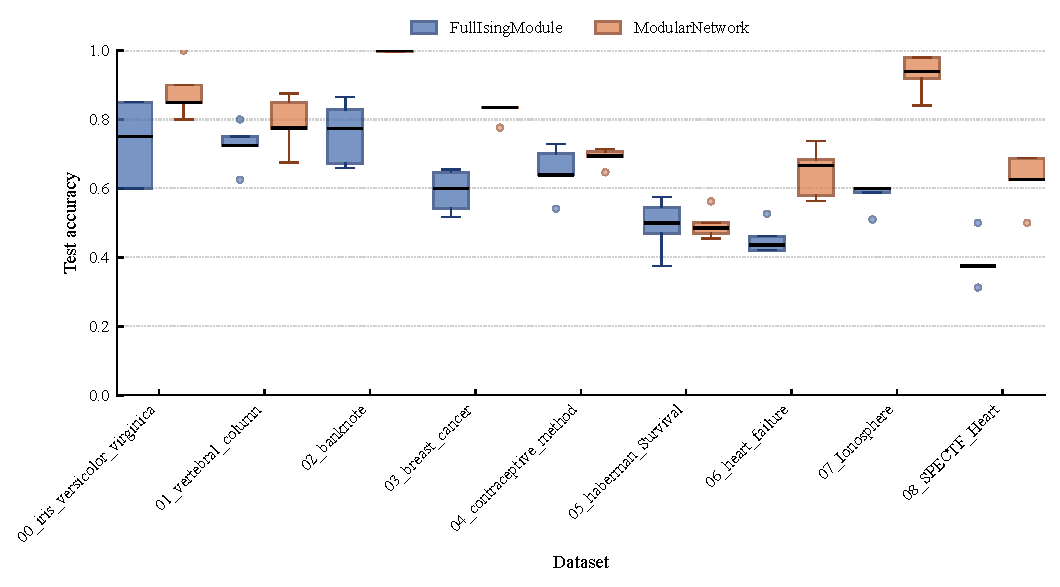
\includegraphics[width=\linewidth]{plots/uci_balanced_combined_boxplot.pdf}
    \caption{Test accuracy on the pre-balanced UCI datasets. Each box aggregates
    the five cross-validation folds for the single Ising module and the Ising
    network.}
    \label{fig:boxplot_balanced}
\end{figure}

\subsubsection{Synthetic XOR Datasets}\label{sec:res_xor}

The last block tests the two architectures on the synthetic
$d$-dimensional XOR family with $d \in \{1,\dots,6\}$.

\begin{table}[H]
\centering
\caption{Performance metrics for the single Ising module on the synthetic
$d$-dimensional XOR problem, for $d \in \{1,\dots,6\}$ (single stratified
train/test split).}
\label{tab:ising_xor}
\begin{tabular}{lcccc}
\hline
Dataset & Accuracy & Precision & Recall & AUC    \\
\hline
XOR-1D  & 0.93     & 0.90      & 0.95   & 0.99 \\
XOR-2D  & 0.84     & 0.83      & 0.85   & 0.92 \\
XOR-3D  & 0.50     & 0.50      & 0.35   & 0.58 \\
XOR-4D  & 0.65     & 0.65      & 0.68   & 0.68 \\
XOR-5D  & 0.51     & 0.50      & 0.84   & 0.53 \\
XOR-6D  & 0.50     & 0.53      & 0.05   & 0.58 \\
\hline
\end{tabular}
\end{table}

\begin{table}[H]
\centering
\caption{Performance metrics for the Ising network on the synthetic
$d$-dimensional XOR problem, for $d \in \{1,\dots,6\}$ (single stratified
train/test split).}
\label{tab:nn_xor}
\begin{tabular}{lcccc}
\hline
Dataset & Accuracy & Precision & Recall & AUC    \\
\hline
XOR-1D  & 1.00     & 1.00      & 1.00   & 1.00 \\
XOR-2D  & 0.98     & 0.95      & 1.00   & 1.00 \\
XOR-3D  & 0.94     & 0.94      & 0.94   & 0.98 \\
XOR-4D  & 0.93     & 0.94      & 0.93   & 0.99 \\
XOR-5D  & 0.86     & 0.85      & 0.87   & 0.93 \\
XOR-6D  & 0.87     & 0.84      & 0.93   & 0.96 \\
\hline
\end{tabular}
\end{table}

The two models separate clearly on this family
(Fig.~\ref{fig:bar_compare_xor}). The single module already struggles at two
dimensions and decays toward chance as the dimension grows, which suggests
that one energy minimization cannot represent the parity structure on its own.
A finer pattern
is visible within the single module: beyond one dimension, the odd-dimensional
instances are harder than their even-dimensional neighbours.
The 3D and 5D
problems sit essentially at chance (accuracy $0.50$ and $0.51$, AUC $0.58$ and
$0.53$), whereas 2D and 4D stay above it ($0.84$ and $0.65$); the 6D case is
the one exception, collapsing to chance as well. A full account of this
even/odd gap would require a dedicated analysis of which parity functions a
single quadratic Ising energy can express, which we leave to future work. The
network, in contrast, resolves the task regardless of parity: it stays well
above chance up to six dimensions, because its parallel modules learn
complementary coupling patterns whose linear combination reconstructs the
higher-order interactions.

\begin{figure}[H]
    \centering
    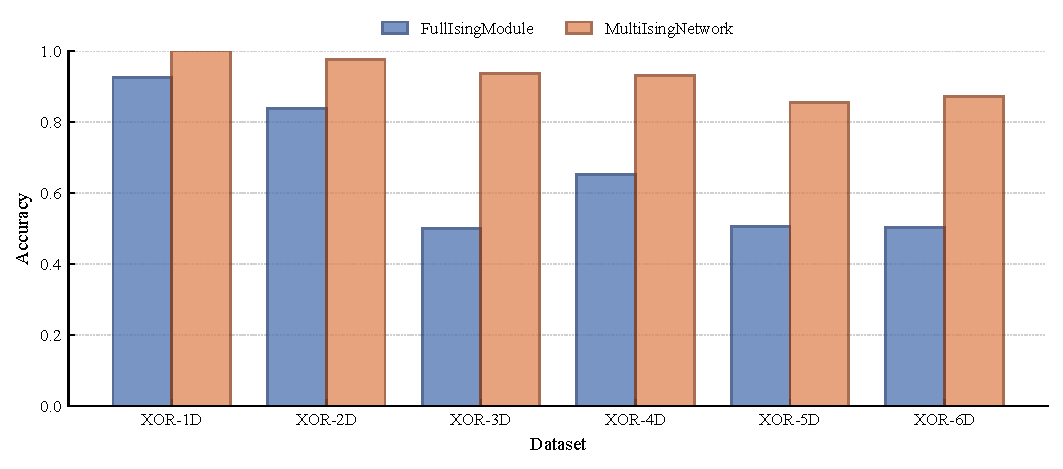
\includegraphics[width=0.95\linewidth]{plots/xor_accuracy_compare.pdf}
    \caption{Mean test accuracy on the synthetic XOR problem as a function of
    the input dimension, for the single Ising module and the Ising network.}
    \label{fig:bar_compare_xor}
\end{figure}

\paragraph{Simulated vs Quantum Annealing}
All experiments reported so far solve the energy minimization with
simulated annealing. As a final test on the 2D instance, we run the
comparison between the single Ising module and a three-module Ising
network ($M = 3$) on two backends: the simulated annealer used above and
a D-Wave quantum processing unit (QPU). QPU resources are only available
on a limited basis, so the experiment replaces the shared
configuration of Table~\ref{tab:hyperparameters} with the reduced
configuration of Table~\ref{tab:qpu-hyperparameters}, applied identically
to both backends. For the same reason the sampling budgets of the two
backends are not matched: the simulated annealer keeps the annealing
schedule of Table~\ref{tab:hyperparameters} (inverse temperature range
$[1,\,10]$, 1\,000 sweeps per read), while the QPU performs a single
anneal-readout cycle per energy evaluation (number of reads equal to one),
the minimum possible QPU time per call, so both the forward energy and
the gradient are computed from the single spin configuration returned by
the hardware. The simulated setting is repeated five times with the seed
held fixed, so that data and initialization are identical across
repetitions and the spread measures only the stochasticity of the
annealer; the quantum setting is run once.

\begin{table}[H]
\centering
\caption{Reduced hyperparameter configuration used for the simulated vs.\
quantum annealing comparison. Shared between the single Ising module and
the three-module Ising network.}
\label{tab:qpu-hyperparameters}
\begin{tabular}{ll}
\hline
Hyperparameter                                   & Value \\
\hline
Dataset                                          & 2D-XOR, 80 points (40 per class) \\
Train/test split                                 & 80/20 \\
Number of epochs                                 & 25 \\
Batch size                                       & 16 \\
Random seed                                      & 42 \\
\hline
Annealer size $n$                                & 8 \\
Ising modules $M$                 & 3 \\
\hline
$\eta_{\Gamma}$                      & $0.01$ \\
$\eta_{\lambda}$                  & $0.02$ \\
$\eta_{\varepsilon}$                     & $0.03$ \\
$\eta_{\text{comb}}$            & $0.02$ \\
\hline
\end{tabular}
\end{table}

The purpose of the comparison is twofold: to check whether the simulated
and the quantum backend lead to comparable outcomes, and to probe how
much the trained performance depends on the quality and completeness of
the annealer output, since the module treats the returned configuration
as the ground state both in the forward energy and in the gradient.
Table~\ref{tab:sim_vs_qpu} reports the test metrics of both models under
both backends.

\begin{table}[H]
\centering
\caption{Test metrics on the 2D XOR problem with the simulated and the
quantum annealing backend. Simulated values are means over five
repetitions with a fixed seed.}
\label{tab:sim_vs_qpu}
\resizebox{\columnwidth}{!}{%
\begin{tabular}{lccccc}
\hline
Model & Accuracy & Precision & Recall & $F_1$ & AUC \\
\hline
\multicolumn{6}{l}{\textit{Simulated annealing}} \\
Single Ising module   & 0.750 & 0.750 & 0.750 & 0.750 & 0.881 \\
Ising network ($M=3$) & 0.938 & 1.000 & 0.875 & 0.933 & 0.984 \\
\hline
\multicolumn{6}{l}{\textit{Quantum annealing}} \\
Single Ising module   & 0.750 & 0.750 & 0.750 & 0.750 & 0.875 \\
Ising network ($M=3$) & 0.938 & 1.000 & 0.875 & 0.933 & 0.984 \\
\hline
\end{tabular}
}
\end{table}

The two backends give the same picture. The Ising network obtains
identical test metrics under simulated and quantum annealing (accuracy
0.938, precision 1.000, recall 0.875, $F_1$ 0.933, AUC 0.984), and the
single module differs only in AUC, where the quantum value (0.875)
coincides with the lower end of the simulated range (0.875--0.891); the
accuracy gap between network and module ($+0.19$) is reproduced on the
hardware. In particular, a single read per energy evaluation is enough
for the QPU trained network to match the result obtained with the
1\,000 sweep simulated schedule, which suggests that training does not
strictly depend on the annealer returning an optimal or exhaustive
solution on this task. These observations rest on one QPU run with one
seed and a 16 point test split, so we take the quantum result as a
reference point, showing that the module and the network train
end to end on quantum hardware, rather than as a statistical claim of
equivalence between the two backends.


\section{Discussion}\label{sec:discussion}

The experiments give a consistent picture. Across the three blocks the
Ising network matches or improves on the single module, and the gap widens
where the task is harder. On the native UCI benchmarks the single module often
reaches an high accuracy by collapsing onto the majority class,
which the precision, recall and $F_1$ columns expose at once. The network
avoids this shortcut on the same datasets: the additional units and the linear
readout give it enough capacity to separate the classes rather than exploit
their prior.

The balanced version confirms this reading. Once the class prior is removed,
the inflated accuracies of the single module disappear and its scores fall to
or below chance on the hardest sets, while the network keeps a clear margin on
breast cancer, ionosphere, heart failure and SPECTF. The single module is thus
more sensitive to class imbalance, and the parallel
composition is what restores a usable decision boundary.
Haberman is the
exception: neither model exceeds chance on it. This agrees with the
literature, where haberman is reported among the hardest UCI sets, its minority
class composed mostly of unsafe (borderline, rare and outlier) examples lying
in the overlap region, so that classifiers drift toward the majority baseline
regardless of the model family~\cite{Napierala2016types}. We therefore
attribute the haberman result to the data rather than to the method.

The synthetic XOR family isolates the same effect under controlled
non-linearity. The single module already struggles in two dimensions and
degrades toward chance as the dimension grows, which suggests that a single
energy minimization cannot represent the parity structure on its own; the
odd-dimensional instances are the hardest, sitting at chance in three and five
dimensions.
The network stays well above chance up to six dimensions, because
the parallel modules learn complementary coupling patterns whose linear
combination reconstructs the higher-order interactions. Since all runs share a
single hyperparameter set, this is the clearest evidence that the gain comes
from the architecture rather than from per-dataset tuning. The reduced 2D XOR
run on quantum hardware adds a practical data point: with a single read per
energy evaluation, both models trained on the QPU match their simulated
counterparts on this task.

A practical remark concerns cost. The dominant expense of the model is the
annealing call. Because the modules act on disjoint spin sets, several of them
can in principle be compiled onto a single physical annealer at once, packing
independent Ising problems into different regions of the qubit graph. This
would amortize the access latency of a quantum processor over many modules and
make wider or deeper Ising networks practical on real hardware.

\section{Conclusion}\label{sec:conclusion}

We presented a differentiable Ising energy module that integrates the
parametric Ising model of Schmid et al.~\cite{10.21468/SciPostPhysCore.7.1.013}
into PyTorch, together with the Ising network, a shallow architecture that
composes several such modules through a trainable linear readout. The module
carries the analytic coupling gradient into automatic differentiation and
behaves as a standard layer, so it can be trained end-to-end with ordinary
gradient-based tooling.

The empirical study supports two conclusions. The single module is expressive
but fragile under class imbalance, where it tends to collapse onto one class,
whereas the network removes this behaviour, improves the metrics and recovers
a meaningful decision boundary on most datasets. On the synthetic XOR problems
the network captures non-linear interactions up to six dimensions while the
single module fails beyond the simplest cases. A reduced 2D XOR experiment on
a D-Wave QPU reproduces the simulated results with a single read per energy
evaluation, showing that both models also train end-to-end on quantum
hardware.

The value of the approach is that an Ising solver becomes a reusable node that
drops into a hybrid architecture and trains within the existing PyTorch
ecosystem, optimizers, loss functions and learning-rate schedulers included.
Placed inside such a network, the module shows the gains expected from added
capacity.
The study has clear
limits: the architecture is shallow, performance rests on a single shared
hyperparameter set rather than per-task tuning, and the benchmark suites were
run with a simulated annealer, with quantum hardware probed only on a reduced
2D XOR configuration. The shared hyperparameter set is a limit in that the
reported scores are likely below the maximum potential of the method, but it
also admits a positive reading: the gains of the Ising network hold without
any per-task tuning, which speaks for the robustness of the architecture.
Future work will explore deeper architectures, the
compilation of multiple modules onto a single physical annealer, and
larger-scale experiments on quantum annealing hardware.

\bibliographystyle{IEEEtran}
\bibliography{bibliography}
\EOD

\end{document}

